\section{Experiment}
\begin{figure*}[t]
    \centering
    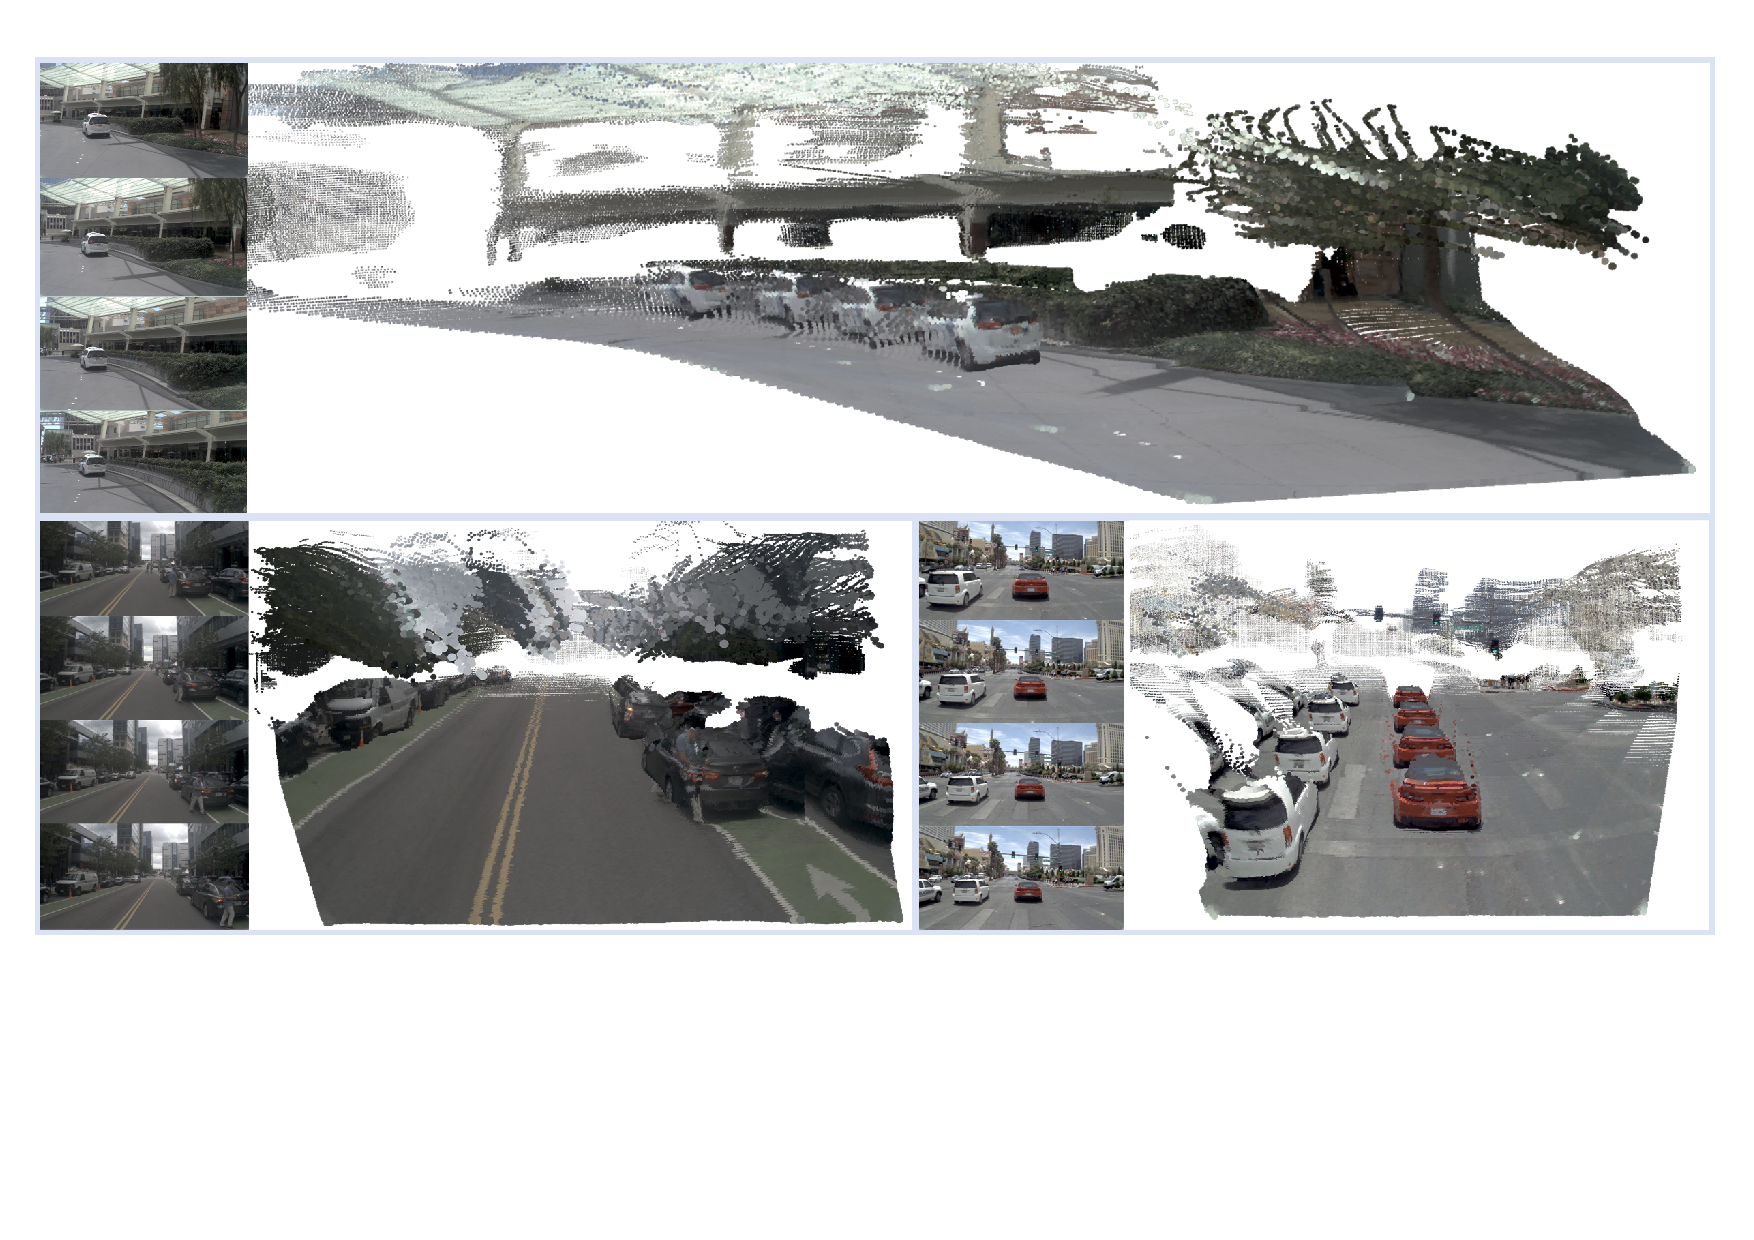
\includegraphics[width=0.98\textwidth]{imgs/3r_recon.pdf}
    \caption{\textbf{Visualization of 4D recontruction results.} The left images are the sequential visual inputs, the right visualized points are the reconstructed geometry. }
    \label{fig_recon_0}
\end{figure*}


\begin{figure*}[t]
    \centering
    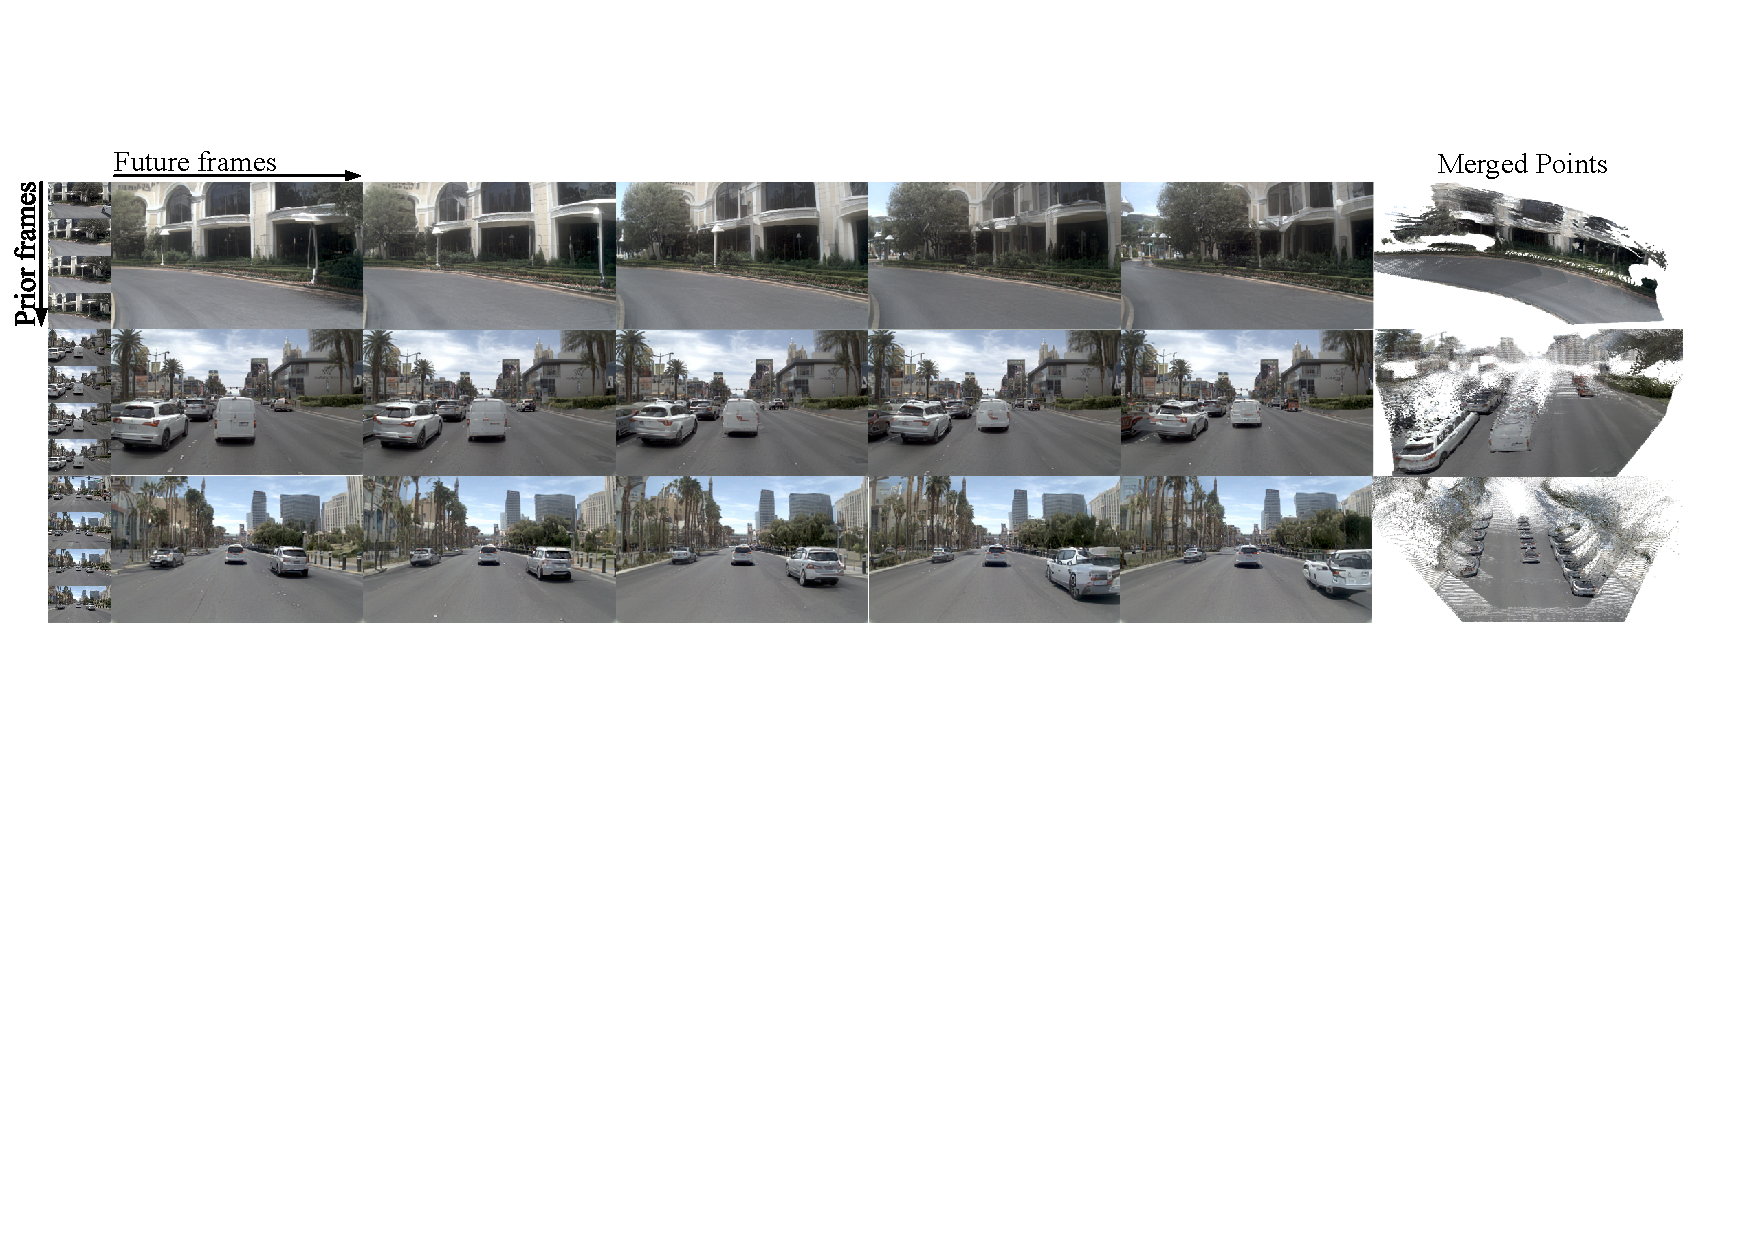
\includegraphics[width=1.0\textwidth]{imgs/gen_res.pdf}
    \caption{\textbf{Visualization of 4D generation results.} Given sequential prior visual frames, UniDWM generates future visual frames with corresponding geometry. We merge the geometries and visualize them as colored points. }
    \label{fig_gen_0}
\end{figure*}

We primarily evaluate our models on the NAVSIM~\cite{navsim} dataset. Details of the dataset and evaluation metrics are provided in Appendix~\ref{dataset_metrics}.

\subsection{Implementation Details}
We utilize DINOv3-B \cite{dinov3} and DCAE \cite{dcae} as the static encoder, separately. The dynamic encoder is composed of $12$-layer spatiotemporal transformers with $170$M parameters. The reconstruction decoders for geometry, appearance, and ego pose are independent and built following \cite{vggt}. We employ a $12$-layer next-frame prediction diffusion transformer with $459$M parameters, and a $16$-layer trajectory prediction diffusion transformer with $33$M parameters. The point and depth map annotations are obtained by projecting the LiDAR points to the image plane. The training recipe is composed of two stages: 1) Reconstruction training, where the model is trained from scratch on the \textit{navtrain} split of the NAVSIM dataset for reconstruction objective $\mathcal{L}_{recon} + \lambda \text{SIGReg}$; 2) Reconstruction and generation joint training, where the model inherits the weights from the first stage training and keeps training with objective $\mathcal{L}_{gen} + \mathcal{L}_{recon} + \lambda \text{SIGReg}$. $\lambda$ was set to $2 \times10^{-4}$ for all experiments. All input images are resized to a resolution of $224 \times 384$ pixels. 50 epochs were performed with a batch size of $64$ for both the first and second stages. The AdamW optimizer was utilized, with a learning rate set to $1 \times 10^{-4}$ and a weight decay of $5 \times 10^{-2}$. In all experiments, the DiT sampling step for the next frame and trajectory were configured to $100$ and $5$, respectively.


% \begin{table}[t]
% \centering
% \begin{tabular}{lccc}
% \toprule
% \textbf{Method} & \textbf{FID$\downarrow$} & \textbf{FVD$\downarrow$} & \textbf{LPIPS$\downarrow$}\\
% \midrule
% % DriveDreamer~\cite{drivedreamer} & 196.2 & 0.153\\
% Epona~\cite{epona} & 182.7 & 0.149 \\
% \textbf{UniDWM (ours)} & \textbf{162.4} & \textbf{0.131} \\
% \bottomrule
% \end{tabular}
% \label{tab:video}
% \caption{\textbf{Video generation results.}}
% \end{table}


\subsection{Experimental Results}


\noindent\textbf{Evaluation of Trajectory Planning.}
We evaluate UniDWM on the NAVSIM \textit{navtest} split and compare it with a wide range of representative trajectory planning methods, including both perception-label-supervised and label-free approaches. As shown in Table~\ref{tab:navsim_pdms}, methods that leverage dense perception annotations generally achieve strong performance, with GaussianFusion~\cite{liu2025gaussianfusion} attaining the best overall results among perception-supervised methods. Focusing on label-free settings, UniDWM demonstrates competitive performance without relying on any perception labels. In particular, UniDWM with a DINOv3-B backbone achieves the best results among all label-free methods, significantly outperforming prior approaches such as raw DINOv3 \cite{dinov3}, Epona~\cite{epona}, and World4Drive~\cite{zheng2025world4drive} across all evaluation metrics. Moreover, comparing UniDWM variants with different encoders highlights the importance of a static encoder with sufficient capacity. Replacing the DCAE encoder with DINOv3-B yields substantial improvements across all metrics, demonstrating that UniDWM can effectively leverage stronger encoders. Overall, these results suggest that UniDWM provides a scalable and annotation-efficient alternative for trajectory planning, narrowing the performance gap between perception label-free and fully supervised methods.



\begin{table}[t]
\centering
\caption{\textbf{4D reconstruction results on the NAVSIM \textit{navtest} split.}}
\begin{tabular}{cccc}
    \toprule
    \textbf{Method} & \textbf{Acc.$\downarrow$} & \textbf{Comp.$\downarrow$} & \textbf{Overall$\downarrow$}\\
    \midrule
    VGGT & 3.764 & 2.236 & 3.000 \\
    Spann3R & 2.028 & 2.202 & 2.115  \\
    UniDWM (ours) & \textbf{1.878} & \textbf{1.575} & \textbf{1.727} \\
    % Ours (Depth + Cam) & $\underline{0.873}$ & $\underline{0.482}$ & $\underline{0.677}$ \\
    \bottomrule
\end{tabular}
\label{tab:3r}
\end{table}

\begin{table*}[t]
\centering
% \resizebox{\linewidth}{!}{
\caption{\textbf{Ablation study} of different architecture configurations. Results are obtained on the NAVSIM \textit{navtest} split. }
\begin{tabular}{cccc|ccccc}
\toprule
\multirow{2}{*}{\textbf{\textit{\shortstack{Ego Pose\\ Reconstruction}}}} & \multirow{2}{*}{\textbf{\textit{\shortstack{Appearance\\ Reconstruction}}}} & \multirow{2}{*}{\textbf{\textit{\shortstack{Geometry \\Reconstruction}}}} & \multirow{2}{*}{\textbf{\textit{\shortstack{Dynamic \\Generation}}}} &\multirow{2}{*}{\textbf{NC$\uparrow$}} & \multirow{2}{*}{\textbf{DAC$\uparrow$}} & \multirow{2}{*}{\textbf{EP$\uparrow$}} & \multirow{2}{*}{\textbf{TTC$\uparrow$}} & \multirow{2}{*}{\textbf{PDMS$\uparrow$}} \\
&&&&&&&&\\
\midrule
\ding{51} & \ding{55} & \ding{55} & \ding{55} & 96.5 & 88.3 & 74.3 & 90.5 & 78.5 \\
\ding{51} & \ding{51} & \ding{55} & \ding{55} & 97.6 & 90.1 & 77.1 & 91.6 & 81.3 \\
\ding{51} & \ding{55} & \ding{51} & \ding{55} & 96.8 & 90.7 & 76.3 & 91.1 & 80.0 \\
\ding{51} & \ding{55} & \ding{55} & \ding{51} & 96.8 & 90.7 & 76.3 & 91.1 & 80.9 \\
\ding{51} & \ding{55} & \ding{51} & \ding{51} & 97.3 & 90.7 & 76.8 & 91.7 & 81.6 \\
\rowcolor{cyan!20}
\ding{51} & \ding{51} & \ding{51} & \ding{51} & 97.3 & 91.6 & 77.4 & 92.1 & 82.4 \\
% \ding{51} & \ding{51} & \ding{51} & \ding{51} & 60M & 98.2 & 96.2 & 94.7 & 82.2 & 88.1 \\
\bottomrule
\end{tabular}
\label{tab:ablation}
\end{table*}

\begin{table}[t]
\centering
\caption{\textbf{Additional finetune with GRPO.} The model in the first row of Table~\ref{tab:ablation} is used as the baseline.}
\resizebox{\columnwidth}{!}{
\begin{tabular}{c|ccccc}
\toprule
\textbf{Method} & \textbf{NC$\uparrow$} & \textbf{DAC$\uparrow$} & \textbf{EP$\uparrow$} & \textbf{TTC$\uparrow$} & \textbf{PDMS$\uparrow$} \\
\midrule
Baseline            & 96.5 & 88.3 & 74.3 & 90.5 & 78.5 \\
Baseline w/ GRPO    & 96.6 & 90.4 & 76.6 & 91.8 & 81.2 \\
UniDWM              & 97.3 & 91.6 & 77.4 & 92.1 & 82.4 \\
UniDWM w/ GRPO      & \textbf{97.4} & \textbf{93.2} & \textbf{80.1} & \textbf{93.3} & \textbf{84.9} \\
\bottomrule
\end{tabular}
}
\label{tab:grpo}
\end{table}

\noindent\textbf{Evaluation of 4D Reconstruction.}
To evaluate the 4D reconstruction capability of UniDWM, we compare it with VGGT~\cite{vggt} and Spann3R~\cite{wang20253d} on the NAVSIM \textit{navtest} split, using Accuracy ($\text{Acc.}$), Completeness ($\text{Comp.}$), and Overall Chamfer Distance ($\text{Overall}$) as metrics. As shown in Table~\ref{tab:3r}, UniDWM achieves the best performance across all metrics, with the lowest Overall ($1.727$), Accuracy ($1.878$), and Completeness ($1.575$). Benefiting from the joint 4D reconstruction (Sec.~\ref{recon}), UniDWM reduces the Overall metric by $\mathbf{42.4\%}$ compared to VGGT, demonstrating its effectiveness in producing high-fidelity and temporally coherent 4D reconstructions. Qualitative results in Figure~\ref{fig_recon_0} further validate these findings. UniDWM reconstructs fine-grained geometric details (e.g., overhead structures and ground markings), maintains strong temporal coherence for dynamic objects (e.g., vehicles), and achieves good scene completeness (e.g., traffic lights). Together, these results confirm the robustness and effectiveness of UniDWM for 4D reconstruction.

\noindent\textbf{Evaluation of 4D Generation.}
Figure~\ref{fig_gen_0} shows the 4D generation results of UniDWM using autoregressive next-frame prediction of both images and point clouds. UniDWM accurately captures the geometry and appearance of static scene elements relative to the ego vehicle, with good alignment between visual content and generated geometry. For dynamic agents, the model preserves reasonable geometric consistency, though visual artifacts may appear over long horizons due to error accumulation from autoregressive inference. This issue arises from the training–inference mismatch and could be mitigated by techniques such as chain-of-forward training \cite{epona}. However, since the primary focus of this work is on the representation learning of driving scenes rather than generation quality optimization, we leave exploration of such techniques to future work.


\subsection{Ablation Study}
To understand the impact of each design choice in UniDWM, we perform a controlled ablation study on the trajectory planning task by incrementally {\textit{Ego Pose Reconstruction}}, {\textit{Appearance Reconstruction}}, {\textit{Geometry Reconstruction}}, and {\textit{Dynamic Generation}} decoders with a shared DCAE encoder \cite{dcae}. The results are shown in Table~\ref{tab:ablation}. When only using the ego pose reconstruction, the PDMS is 78.5. Introducing {\textit{Appearance Reconstruction}}, {\textit{Geometry Reconstruction}}, and {\textit{Dynamic Generation}} leads to +2.8, +1.5, and +2.4 gains in PDMS, respectively. Combining {\textit{Geometry Reconstruction}} and {\textit{Dynamic Generation}} further improves the performance to $81.6$ PDMS. The best overall performance is achieved when combining all reconstruction and generation decoders. These findings confirm that our multifaceted representation learning strategy effectively captures complementary aspects of the driving scene, where appearance, geometry, and dynamics provide mutually reinforcing supervision signals. 

To further explore the useful planning-oriented information encoded in the latent world representation, we freeze the UniDWM encoder and finetune the trajectory decoder using the GRPO algorithm \cite{li2025recogdrive}. As reported in Table~\ref{tab:grpo}, UniDWM without GRPO already achieves competitive or superior performance compared to the GRPO-enhanced baseline. When GRPO is applied to UniDWM, the model achieves the best overall results, suggesting that the benefits of unified latent world modeling and policy optimization are complementary rather than redundant. These results highlight that high-quality latent world modeling not only improves planning performance directly but also enables effective reinforcement-based finetuning. Additional smoothness analysis of representations is in Appendix~\ref{sec:appendix_smoothness}. 
